\section{Access Network Deployment Algorithm and Evaluation}
\label{sec:winmee}

In this section, we study the access tier network deployment and propose our measurement-driven MAPE framework with the dynamics 
of WiFi and white space bands. We further apply our MAPE framework with the measurements shown in Section~\ref{sec:measurements}
to investigate the access tier gain of WhiteMesh in reducing the number of access point in the Dallas-Fort Worth metroplex.

\subsection{Access Network Model and MAPE} 
\label{subsec:winmeemodel}


% Discuss the white space band in access and backhaul
% Traffic demand calculation
Access tiers must satisfy both the coverage and capacity constraints to provide service for users.
The coverage constraint is from the propagation range of wireless signals and could be calculated 
according to the propagation model of Eq.~\ref{eq:friis}. 
Generally, a coverage of $95\%$ of access tier is acceptable for wireless access 
networks~\cite{robinson2010deploying}. We represent the capacity 
constraint according to the demand of a service area, which could be calculated as the 
summation of individual demands over the service area $D_a=\sum\limits_{p\in P} D_p$. Since household demand 
for the Internet has been previously characterized~\cite{rosston2011household}, $D_a$ could be estimated by the 
population distribution $f$ and service area $k$ as $D_a=\sum\limits_{f \in F,k \in K}\bar{D_p}*f*k$. The capacity 
constraint could be represented with an access point set $M$ according to:
\begin{equation}
\label{eq:nlbound}
\sum_{m \in M}\delta_r^m \ge \sum_{f \in F,k \in K}\bar{D_p}*f*k
\end{equation}

% Discuss the application of activity level
Through the measured activity level, the achieved channel capacity $\delta_r$, could be calculated through the
free time according to:
\begin{equation}
\label{eq:intercap}
\delta_r=\delta*(1-\bar{A})
\end{equation}
Where, the capacity of a clean channel is denoted by $\delta$ under the protocol model which make hard decision 
according to the received signal strength~\cite{gupta2000capacity}. 
With the achieved channel capacity, we could further estimate the capacity of an access point in the access 
tier and link capacity in the backhaul tier.
Further, the radius $R_{QoS}$ satisfy the users traffic demand of the area is estimated from $\delta$ and $D_a$ 
according to the service area shape.

In a joint white space and WiFi scenario, the activity level varies according to various interfering sources 
and the propagation characteristics induced by the environmental characteristics of the service area. A 
simple method with the least number of access points to cover an area is to use multiple orthogonal 
lower-frequency channels. However, the FCC limits white space band availability for data networks in most 
metropolitan areas in the United States~\cite{googledatabase}. Moreover, the number of channels in each band 
is limited. Too many lower-frequency channels will cause high levels of intra-network interference, 
which will be discussed in the next backhaul tier section. We assume that the cost of the network is proportional to the 
number of access points required for a given user demand (i.e., due to the cost of hardware and installation). 
Therefore, given a geographical region for a new network deployment, we build a measurement-driven framework 
called Multiband Access Point Estimation (MAPE) to compute the required number of access points.


\begin{algorithm}[t]
\small
\caption{Multiband Access Point Estimation (MAPE)}
\label{algorithm:mape}
\begin{algorithmic}[1]
\REQUIRE  ~~\\
$A$: Measured Activity Level \\
$F$: Population Distribution\\
$C$: Clean Channel Capacity\\
$n$: Path Loss Exponent \\
$B$: Available Frequency Bands\\
$M$: Area to be Covered
\STATE Split $M$ in to different type, calculate the traffic demand density $f$
\STATE Calculate in-field channel capacity $\delta_r$ as $\delta(1-A)$
\STATE Get the propagation coverage area radius $R_p$ from the Friis model based on $n,B,F$
\STATE Calculate the QoS coverage radius $R_{QoS}$ of a multiband access point that satisfies the demands of the area
\STATE The coverage radius of a multiband access point is $min\{R_p,R_{QoS}\}$ according to Eq.~\ref{eq:nlbound} and Eq.~\ref{eq:friis}.
\STATE Apply a regular-hexagonal deployment to get the number of access points for serving given area $M$
\ENSURE ~~\\
The number of access points\\
\end{algorithmic}
\end{algorithm}

In the spatial domain, the advantage of higher-frequency channels is the spatial reuse, while the lower-frequency 
channels provide greater levels of coverage. Generally, higher frequencies are more appropriate for populated 
areas, and lower frequencies are more appropriate for sparse areas. The temporal variation of spectrum utilization 
differs across bands. For an Internet service provider, the service quality which maps to the capacity constraint 
must be satisfied. Given a metropolitan area, the population distribution can be found according to census data~\cite{uscensus}. 
Then, we estimate the capacity demand of each type of area with the assumption that users 
will exhibit average demand. According to the population distribution, we split the area into different types, 
downtown, residential, and suburban which compose the spatial input. 
We have an average 
channel capacity of each band according to the activity level from Section~\ref{sec:measurements}. 
With the received signal strength threshold, the 
Quality-of-Service-constrained according to Eq.~\ref{eq:nlbound} coverage area of different types per channel, and the spatial reuse distance can be 
directly computed. Then, the service area of an access point could cover can be calculated as the minimal area of the 
QoS-based coverage area and propagation coverage. Then, the transmission power is adjusted to fulfill the coverage 
restriction subject to the FCC regulations for maximum-allowable transmit power. A regular-hexagonal deployment 
process is employed to place the access points. 

\subsection{Results and Analysis}
\label{subsec:winmeeresult}

We use the measurement-based activity levels shown in Table~\ref{tab:activitymeasurement} as an input to 
Alg.~\ref{algorithm:mape}. We specifically use the Millsap sparse area, Millsap downtown, Weatherford residential, 
Dallas residential, and Dallas downtown measurements as inputs of activity level for a given population density. 
Other types of areas could be quantified by more measurements.
We then 
calculate the number of access points for covering a single type 13 km $\times$ 13 km area, varying the population density. The 
output is shown in Fig.~\ref{fig:redensity_winmee}. 

   \begin{figure}
   %\vspace{-0.0in}
   \centering
   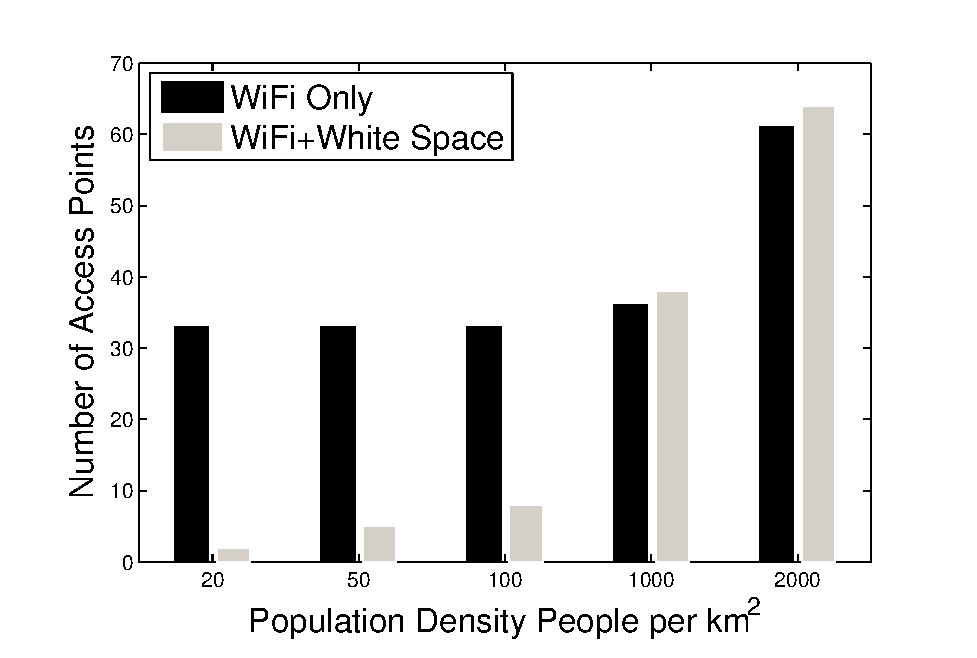
\includegraphics[width=84mm]{figures/redensity_winmee}
   \vspace{-0.1in}
   \caption{Number of Access Points Needed for a 13 km x13 km Area.}
   \label{fig:redensity_winmee}
   \vspace{-0.1in}
   \end{figure}

% Experiment Results & expect results
In the calculation, 
we have the configuration the same as in Section~\ref{sec:problemformulation}.
%we set the demand requested per user to be 2 Mbps with the population density of 20, 50, 100, 1000, 
%and 2000 users per square kilometer. We assume 30\% of the residents will use this service (i.e., the take rate is 
%30), 
We set the population density of 20, 50, 100,1000, and 2000 users per square kilometer.
The maximum transmit power is 30 dBm, with a path loss exponent of $3.5$~\cite{meikle2012global}. From Eq.~\ref{eq:friis}, 
we see that the propagation range is proportional to the wavelength with 450 MHz having a propagation 
range of $11.6$ times that of 5.2 GHz. We adopt an 802.11n maximum data rate of 600 Mbps. For the WiFi+White Space 
scenario, we use 3 channels in each of the 450 MHz, 2.4 GHz and 5.2 GHz bands. For the WiFi Only scenario, we assume 
6 non-overlap channel in the 2.4-GHz band, and 3 channels in the 5.2-GHz band since 2.4 GHz has a greater propagation range than 5.2 GHz. 
Each of these scenarios have the same channels in total (9). As shown in Fig.~\ref{fig:redensity}, with the same number 
of channels, the WiFi+White Space scenario reduces the number of access points by $1650\%$ compared to the WiFi Only scenario in the 
20 people per square km scenario, $660\%$ in the 50 people per square km, and $412.5\%$ in the 100 people per square km 
scenario. The large propagation range of the white space bands is approximately 10 times that of the WiFi bands, creating 
an opportunity for greater coverage. However, as the population density increases, due to the capacity constraint of 
servicing users in the area, the lower-frequency white space bands lose their advantage of larger communication range due 
to the reduction in achievable spatial reuse. At the same time, the activities of other signal sources, such as TV stations 
in downtown areas, reduce the capacity of white space bands. As a result, the WiFi+White Space scenario performs worse 
than the WiFi Only scenario. If we were to count the intra-network interference as in the following section, the situation could become 
even worse. Moreover, FCC has stricter policies on white spaces in urban areas. Fewer channels are available in the 
downtown and urban areas, which makes WiFi a better option for these dense areas.

To understand the influence of band combinations on network deployments, we calculate the number of access points in the 
area when selecting 500 people per square km with a downtown Weatherford spectrum utilization and 1500 people per square 
km with a residential Dallas spectrum utilization. We assume the total number of channels is 12. We use the same setup 
as the previous experiment.
 
 \begin{table}[h]
 \centering
 \begin{tabular}{|c|c|c|c|}
 \hline
 \multirow{2}{*}{No. of Bands} & \multirow{2}{*}{Bands Combination} & \multicolumn{2}{c|}{No. of AP} \\
 \cline{3-4}
  &  & 500 & 1500 \\
 & (Hz) & $ppl/km^2$ &  $ppl/km^2$ \\
 \hline
 \multirow{4}{*}{1}    & 450 M  & 12  & 35 \\
 \cline{2-4}
                              & 800 M & 10  &  30 \\
 \cline{2-4}
			      & 2.4 GHz & 33  &  37 \\
 \cline{2-4}
                              & 5.2 G & 193 &  193 \\ 
 \hline
 \multirow{6}{*}{2}   & 450 M,800 M & 11  & 32\\
 \cline{2-4}
                              & 450 M,2.4 G & 23  & 36\\
 \cline{2-4}
			      & 450 M,5.2 G & 23  & 69\\
 \cline{2-4}
			      & 800 M,2.4 G & 20  & 33\\ 
 \cline{2-4}
			      & 800 M,5.2 G & 20  & 59\\ 
 \cline{2-4}
			      & 2.4 G,5.2 G & 33  & 73\\ 
 \hline
 \multirow{4}{*}{3} & 450 M,800 M,2.4 G & 16  & 33\\
 \cline{2-4}
                              & 450 M,800 M,5.2 G & 16  & 48\\
 \cline{2-4}
			      & 450 M,2.4 G,5.2 G & 33  & 53\\
 \cline{2-4}
			      & 800 M,2.4 G,5.2 G & 30 &  49\\ 
 \hline
 4  & 450 M,800 M,2.4 G,5.2 G & 21  & 44 \\
 \hline
 \end{tabular}
 \caption{Channel Allocations for $500$ and $1500$ Population Density Scenarios}
 \label{tab:500comb}
 \vspace{-0.4in}
 \end{table}


In Table~\ref{tab:500comb}, we compare the number of access points with 12 channels through all 
the possible combinations of bands to leverage the activity level and propagation impacts on the 
access tier deployment. 
% Single band compare
Since purchasing and deploying access points is the primary cost of a wireless 
infrastructure, to simplify the calculation, we only count the number of access points as 
the network's cost. 
When all the channels are in the same band, as the frequency goes up, more access 
points are needed to serve the area due to the limited propagation range. However,
450 MHz does not outperform 800 MHz with a single band at both the 500 and 1500 people per
square km cases because 450-MHz channels have larger measured activity levels. 
White space band channels outperform WiFi bands by up to 1830\% in the single band case
with 500 people per square km, but with 1,500 people per square km, the cost reduction
decreases to only 543\%.
% Two bands 
We now distribute an equal number of channels to two-band combinations and run the experiments 
with the same population densities and spectrum utilization represented by activity level. 
The results show that the white space band
combination (450 and 800 MHz) performs better than WiFi only (2.4 and 5.2 GHz) by 200\% and
128\% with the people per square km of 500 and 1,500, respectively. In fact, the white space only
scenario (450 and 800 MHz) has almost the same performance as the scenarios with one white band and
one WiFi band (450 MHz and 2.4 GHz; 800 MHz and 2.4 GHz) with 1,500 people per square km.
However, with 500 people per square km, the white space only scenario is much better than any other two-band combination.
% Three bands
White space channels provide up to 87.5\% cost reduction in three-band combination scenarios with
500 people per square km, and up to 33.3\% with 1,500 people per square km.  With four bands,
the number of access points required does not reduce using white space bands.

From Fig.~\ref{fig:redensity_winmee} and Table~\ref{tab:500comb}, we show that 
the reduction in number of access points satisfy the users traffic demand varies 
as the population density increases. Note that a more optimal allocation of channels in different bands could offer
further cost reductions. We further show that as population and activity level increase, 
at some point, the performance of white space only scenario could be the same as a combination of
white space and WiFi bands. 

